\documentclass[format=acmsmall, review=false, natbib=false]{acmart}
\usepackage{acm-ec-23}
\usepackage{booktabs} % For formal tables
\usepackage[ruled]{algorithm2e} % For algorithms
\renewcommand{\algorithmcfname}{ALGORITHM}
\SetAlFnt{\small}
\SetAlCapFnt{\small}
\SetAlCapNameFnt{\small}
\SetAlCapHSkip{0pt}
\IncMargin{-\parindent}

%Imports biblatex package
\usepackage[backend=biber]{biblatex}
\addbibresource{ref.bib} %Import the bibliography file
\usepackage{amsthm}

\newtheorem{definition}{Definition}[section]
\newtheorem{theorem}{Theorem}[section]
\newtheorem{corollary}{Corollary}[theorem]
\newtheorem{lemma}[theorem]{Lemma}
\newtheorem{proposition}[theorem]{Proposition}

\usepackage{tcolorbox}
\tcbuselibrary{breakable}

% Choose a citation style by commenting/uncommenting the appropriate line:
%\setcitestyle{acmnumeric}
%\setcitestyle{authoryear}

% Title. Note the optional short title for running heads. In the interest of anonymization, please do not include any acknowledgements.
\title{Double Auction on Social Network}

% Anonymized submission.
\author{Huizhe Su (2020533009), Cheng Peng (2020533068), Jingtian Hu (2020533167)}

% Abstract. Note that this must come before \maketitle.
\begin{abstract}
	In this project, we explored the mechanisms on double auction in network. With three different constraints on buyer networks, we made three different attempts: Resale mechanism with Leave and Share, DNA with Graph Partition and Club Auction. The first attempt is proved that sellers will play truthfully but buyer will not be IC, while the property for the second attempt remains an open question. We also gave a proof to show that our third mechanism is IC.
\end{abstract}

\begin{document}

% Title page for title and abstract only.
% \begin{titlepage}

\maketitle

% \end{titlepage}

% Paper body
\section{Introduction}

The establishment of huge social network such as Tiktok, Wechat and Weibo has brought both challenges and opportunity.
Leveraging the connectivity of social network to promote social welfare has become a fruitful area of study in algorithmic game theory research, particularly since the publication of \cite{mechanism-design-in-social-network} in 2017.

In this project, we study the double auction mechanisms in a social network. Double auction is a process to try to match multiple buyers and sellers. In traditional double auction mechanism, network structure are usually ignored. However, double auction on social network is a more general and practical. Bringing social network into a double auction creates a lot of new challenges since the participants are both cooperator and competitor. The main difficulty will be to design a mechanism that incentives participants to invite each other and report their type truthfully. Our project focus on scenario that only buyers forms a social network and has explored three mechanisms with different restrictions on the buyer networks.


\section{Related work}

Since IDM\cite{IDM} was coined, various of social network based auction mechanisms have been developed.
We introduce a few typical mechanisms that are pertinent to our problem. \ref{tab:previous-works} gives a summary of them.

\begin{table}[H]
	\centering
	\begin{tabular}{ll|l|l}
		players   & supply         & restriction           & mechanism \\
		\hline
		one-sided & single item    & arbitrary network     & IDM       \\
		one-sided & multiple items & arbitrary network     & MUDAN     \\
		two-sided & single item    & disjoint buyer groups & DNA       \\
	\end{tabular}
	\caption{summary of typical social network auction mechanisms}
	\label{tab:previous-works}
\end{table}

% \cite{DNA} is the only paper that covers double auctions on a network. However, the mechanism proposed has a strong restriction on the buyer social network. It requires buyer networks are separated into several
% disjoint subgroups, and all subgroups has one head buyer who knows the auction initially.
% Therefore, we need to derive a mechanism that works for more general network structures.

\subsection{IDM}

IDM\cite{IDM} is a mechanism for a single source to sell a single item.
It includes a critical value payment and leverages local reselling to implement the allocation.\par
IDM is IR, IR and WBB, which are all the achievable properties when efficiency is discarded.

\subsection{MUDAN}

MUDAN/MUDAR\cite{MUDAN-MUDAR} is designed to solve the multi-item auction problem.
That is, a seller wants to sell a bunch of homogeneous items to others and each potential buyer is willing to purchase at most one item.
MUDAN defines the priority of an agent to be the number of agents invited by it.
The mechanism explores the graph in iterations, determining allocation and payment in the meanwhile.\par
MUDAN achieves IC, IR and WBB. \cite{MUDAN-MUDAR} also established a $1/m$ efficiency property.

\subsection{DAN}

DNA\cite{DNA} is the only one existing double auction mechanism.
It leverages McAfee's mechanism to determine the allocation and uses a VCG-alike payment scheme, achieving IC, IR and WBB.\par
However, DNA assumes that the buyer groups, i.e., the subnetworks rooted at each head buyer are disjoint. This is unlikely in real-world social networks.

\subsection{Limitations of Existing works}

We can see that existing mechanism failed to make a truthful two-sided trade happen in general social network. Our work aims to design a mechanism with incentive compatibility property for such scenario.

\section{Model}

Consider a double auction market of $n+m$ participants
where $n$ out of them are sellers and the rest $m$ participants are potential buyers. Let $S=\{s_1,s_2,\ldots, s_n\}$ and $B=\{b_1,b_2,\ldots b_m\}$ be the set of all sellers and buyers.
Each seller $s_i\in S$ is holding a one-unit item and is willing to sell it at price no lower than $v^s_i$. Each buyer $b_j\in B$ wants to purchase one item with price no more than $v^b_j$.

In the social network, each buyer $b_j$ knows a subset of other buyers $N(b_j)\subseteq B$ and each seller $s_i$ knows a subset of other sellers $N(s_i)$.
Initially, only part of the sellers and buyers, called the heads, are aware of the incoming trade.
The head buyers and head sellers are denoted by $HB$ and $HS$.
Each head buyer $b\in HB$ knows some head sellers $NS(b) \subseteq HS$.
Similarly, each head seller $s\in HS$ knows a proportion of the head buyer $NB(s) \subseteq HB$.

To sell the item at higher price, the sellers want to invite potential buyers other than the initial ones i.e, the head buyers, to expand the auction.
However, once neighboring potential buyers are invited to the auction, they will compete with the initial buyers for the items. Intuitively, a buyer has incentive to keep his neighboring buyers from entering the market.
Therefore, the market owner must adopt a mechanism encouraging the buyers in the market to inform the neighbors not being aware of the auction.

A mechanism for double auction on social network requires the buyers and the sellers to report their private information and decide the allocation of items and payment for each agent.
For the sellers, the mechanism asks them to reveal their expected price $\hat v^s=(\hat v^s_1,\hat v^s_2,\ldots \hat v^s_n)$.
The mechanism also requires the buyers to report their type $\hat\theta_i = (\hat v^b_i, \hat r_{s_i})$ and use $\hat\theta = (\hat\theta_1,\hat\theta_2,\ldots,\hat\theta_m)$ to denote a reported type profile.

After receiving the reported information $\hat\theta$ and $\hat v^s$, the mechanism determines the allocation $\pi^s,\pi^b$ and the payment $p^s,p^b$.
\begin{itemize}
	\item For each seller $s_i$:
	      The allocation $\pi^s_i = 1$ means that he can trade the item with a buyer, otherwise $\pi^s_i = 0$.
	      The payment $p^s_i\leq 0$ gives the money $s_i$ can get from the market owner.
	\item For each buyer $b_i$:
	      The allocation $\pi^b_i = 1$ indicates that he get one item from a seller, while $\pi^b_i=0$ if he gets no item.
	      The payment $p^b_i>0$ if $b_i$ is asked to pay money to the market owner
	      and $p^b_i<0$ when $b_i$ can get some rewards from the market owner.
\end{itemize}


We make a few definitions of properties for further discussion.

\begin{definition}[active buyers]
	Given a profile $\hat\theta$, we say buyer $b_i$ is active
	if there exists $q_1,q_2,\ldots q_k$ such that
	$b_{q_1}\in H$ is a head buyer, $b_{q_k}=b_i$ is the active buyer and
	$b_{q_{i+1}} \in \hat r_{b_{q_i}}$ for every $i=1,2\ldots k-1$.
	That is a buyer is active if he is a head buyer or an active buyer invites him.\\
	Let $Q\subseteq B$ be the set of all active buyers.
\end{definition}

Next we definition the desired properties of the mechanism.

\begin{definition}[valid]
	A mechanism is valid if for all possible input of $(\hat\theta,\hat v^s)$ the following conditions are satisfied.
	\begin{itemize}
		\item If $b_i\not\in Q$ then $\pi^b_i=p^b_i=0$.
		\item $\sum_{b_i\in B} \pi^b_i = \sum_{s_i\in S} \pi^s$.
	\end{itemize}
\end{definition}

\begin{definition}[utility]
	The utility is the welfare an agent gains from participating the trade.
	\begin{itemize}
		\item For $b_i\in B$, his utility is $u^b_i = \pi^b_i v^b_i-p^b_i$.
		\item For $s_i\in S$, his utility is $u^s_i = \pi^s_i v^s_i-p^s_i$.
	\end{itemize}
\end{definition}

\begin{definition}[individual rational (IR)]
	A mechanism is IR if for all possible input of $(\hat\theta,\hat v^s)$,
	\begin{itemize}
		\item For all $b_i\in B$, $u^b_i((\theta_i,\hat\theta_{-i}),\hat v^s)\geq 0$.
		\item For all $s_i\in S$, $u^s_i(\hat\theta,(v^s_i, \hat v^s_{-i})\geq 0$.
	\end{itemize}
	That is, no agent is punished for participating truthfully.
\end{definition}

\begin{definition}[incentive compatible (IC)]
	A mechanism is IC if
	\begin{itemize}
		\item For all $b_i\in B$,
		      $u^b_i((\theta_i,\hat\theta_{-i}),\hat v^s)
			      \geq u^b_i(\hat\theta,\hat v^s)$.
		\item For all $s_i\in S$,
		      $u^s_i(\hat\theta,(v^s_i,\hat v^s_{-i}))
			      \geq
			      u^s_i(\hat\theta,\hat v^s)$
	\end{itemize}
	That is, an agent's utility is maximized when he participates truthfully.
\end{definition}

\begin{definition}[weak budget balance (WBB)]
	A mechanism is WBB if
	$\sum_{s_i\in S} p^s_i(\hat\theta,\hat v^s)
		+\sum_{b_i\in B} p^b_i(\hat\theta,\hat v^s) \geq 0$
	for all $(\hat\theta,\hat v^s)$.
	That is, the market owner never pay extra money for running the mechanism.
\end{definition}

\begin{definition}[budget balance (BB)]
	A mechanism is BB if
	$\sum_{s_i\in S} p^s_i(\hat\theta,\hat v^s)
		+\sum_{b_i\in B} p^b_i(\hat\theta,\hat v^s) = 0$
	for all $(\hat\theta,\hat v^s)$.
	That is, the market owner returns all the money he collected from the participants.
\end{definition}

\section{Technical Approach}

We have made several attempts to adapt existing mechanisms into our model.

\subsection{Resale mechanism with leave and share}
In double-auction, we want people with high valuations to hold the item. Therefore, resale mechanisms are better than
layer-based mechanisms. Buyers with higher evaluations have more chances to get the item, while buyers with lower
evaluations are rewarded if they invite someone who gets it. From this insight, we designed a naive
resale mechanism that combined IDM with leave and share. The mechanism is described as follows,
\begin{tcolorbox}[title=Algorithm: Resale mechanism with Leave and Share - 1]
	\begin{enumerate}
		\item Sort the sellers in order of their price from lowest to highest.
		\item Let the seller with the lowest price sell the item using IDM. Other sellers are viewed as buyers with 0 valuations.
		\item The seller and the winner leave the network and share their connection.
		\item Repeat step 2, 3 until no seller can sell the item.
	\end{enumerate}
\end{tcolorbox}
However, this mechanism is not IC since the seller with a lower price has more chance to sell their
item at a high price, and the seller has the incentive to misreport a lower price. In the following example, if \(s_1\)
\(s_2\) both report truthfully, then \(s_2\) will receive \(9\). But
if he misreports \(2\), he will receive \(10\)(Fig \ref*{fig:IDMCounter1}). Therefore, he has the incentive to misreport.
\begin{figure}[htbp]
	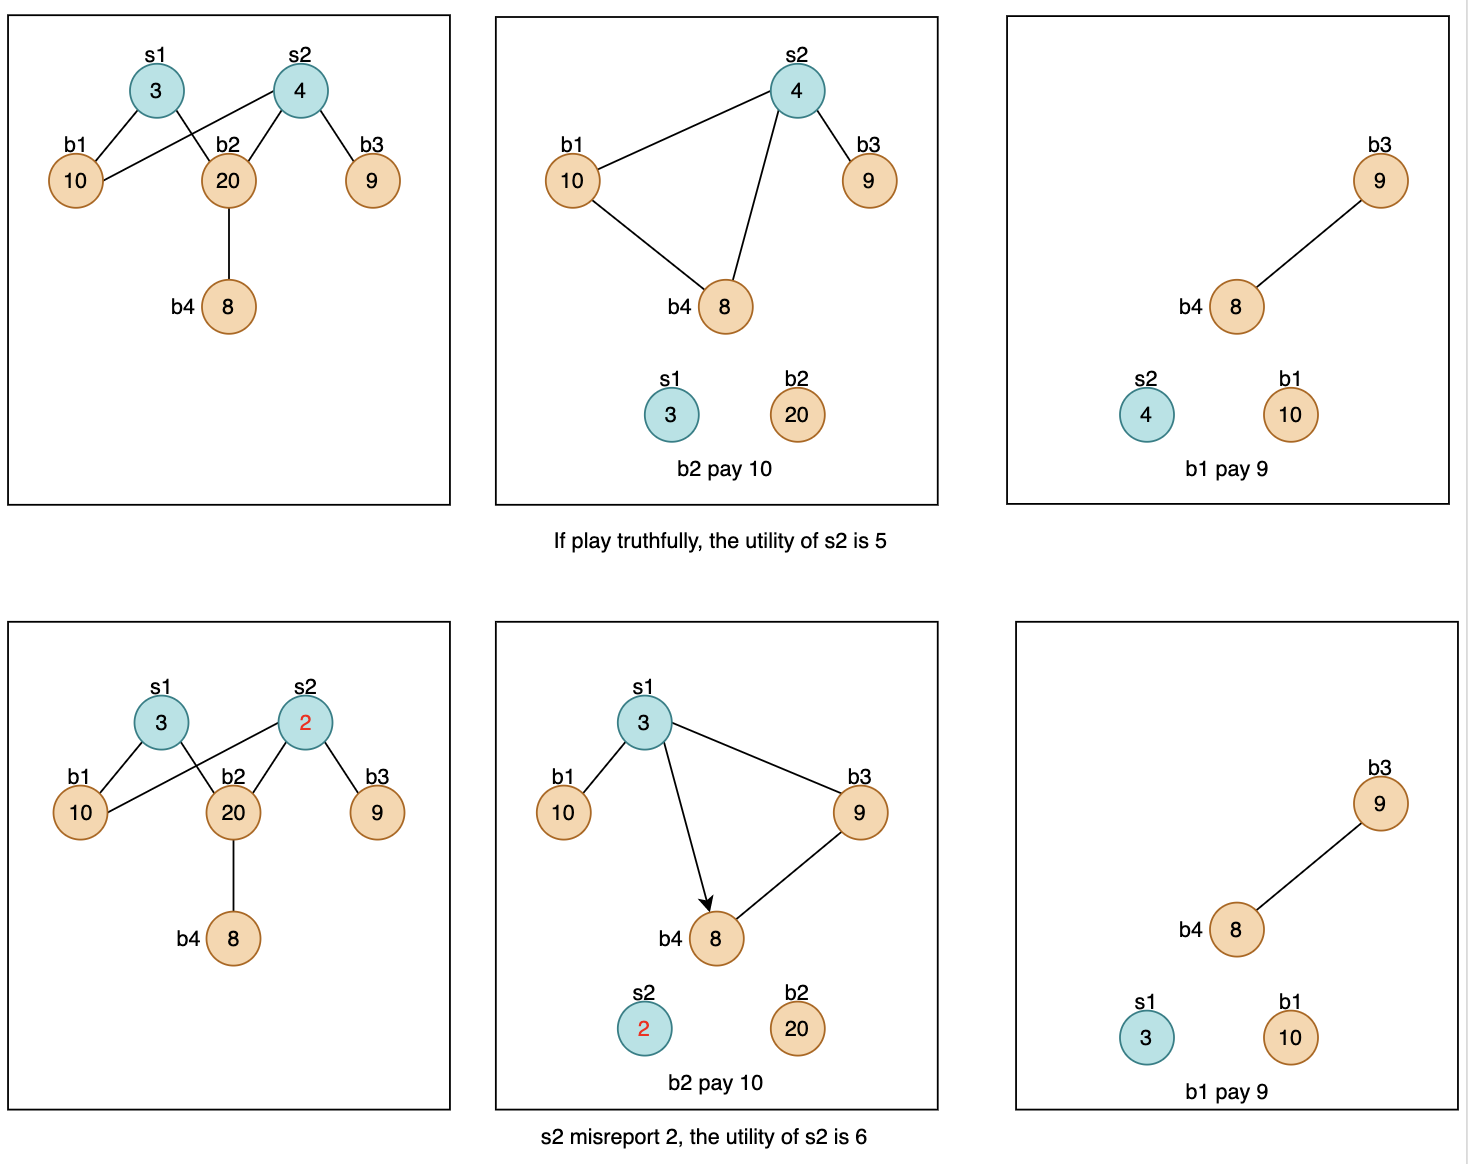
\includegraphics[width=\textwidth]{image/IDMCounter1.png}
	\caption{A run of the naive algorithm}
	\label{fig:IDMCounter1}
\end{figure}

Then we modified the original algorithm. The main idea is still the same, but when calculating
the price using IDM, we first eliminate the highest \(m\) bids, where \(m\) is the number of unmatched sellers.
\begin{tcolorbox}[title=Algorithm: Resale mechanism with Leave and Share - 2]
	\begin{enumerate}
		\item Sort the seller in ascending order and the buyer in descending order.
		\item \emph{Let \(m = \) the number of the remaining seller}
		\item Run IDM. When calculating the payment, omit the \emph{first \(m\) higher bids}.
		\item If the payment is higher than the first seller's expectation, the seller is matched.
		      Otherwise, stop.
		\item The winner leave the network and share its connection.
		\item Go to 2.
	\end{enumerate}
\end{tcolorbox}
As a result, the seller cannot profit more by misreporting. However, this mechanism is still not IC. A buyer who serves as a critical node in the buyer network can get more resale reward by misreporting. Shows in Fig. \ref{fig:IDMcounter2}, buyer can misreport 7 to get a resale reward, then get the item.
\begin{figure}
	\centering
	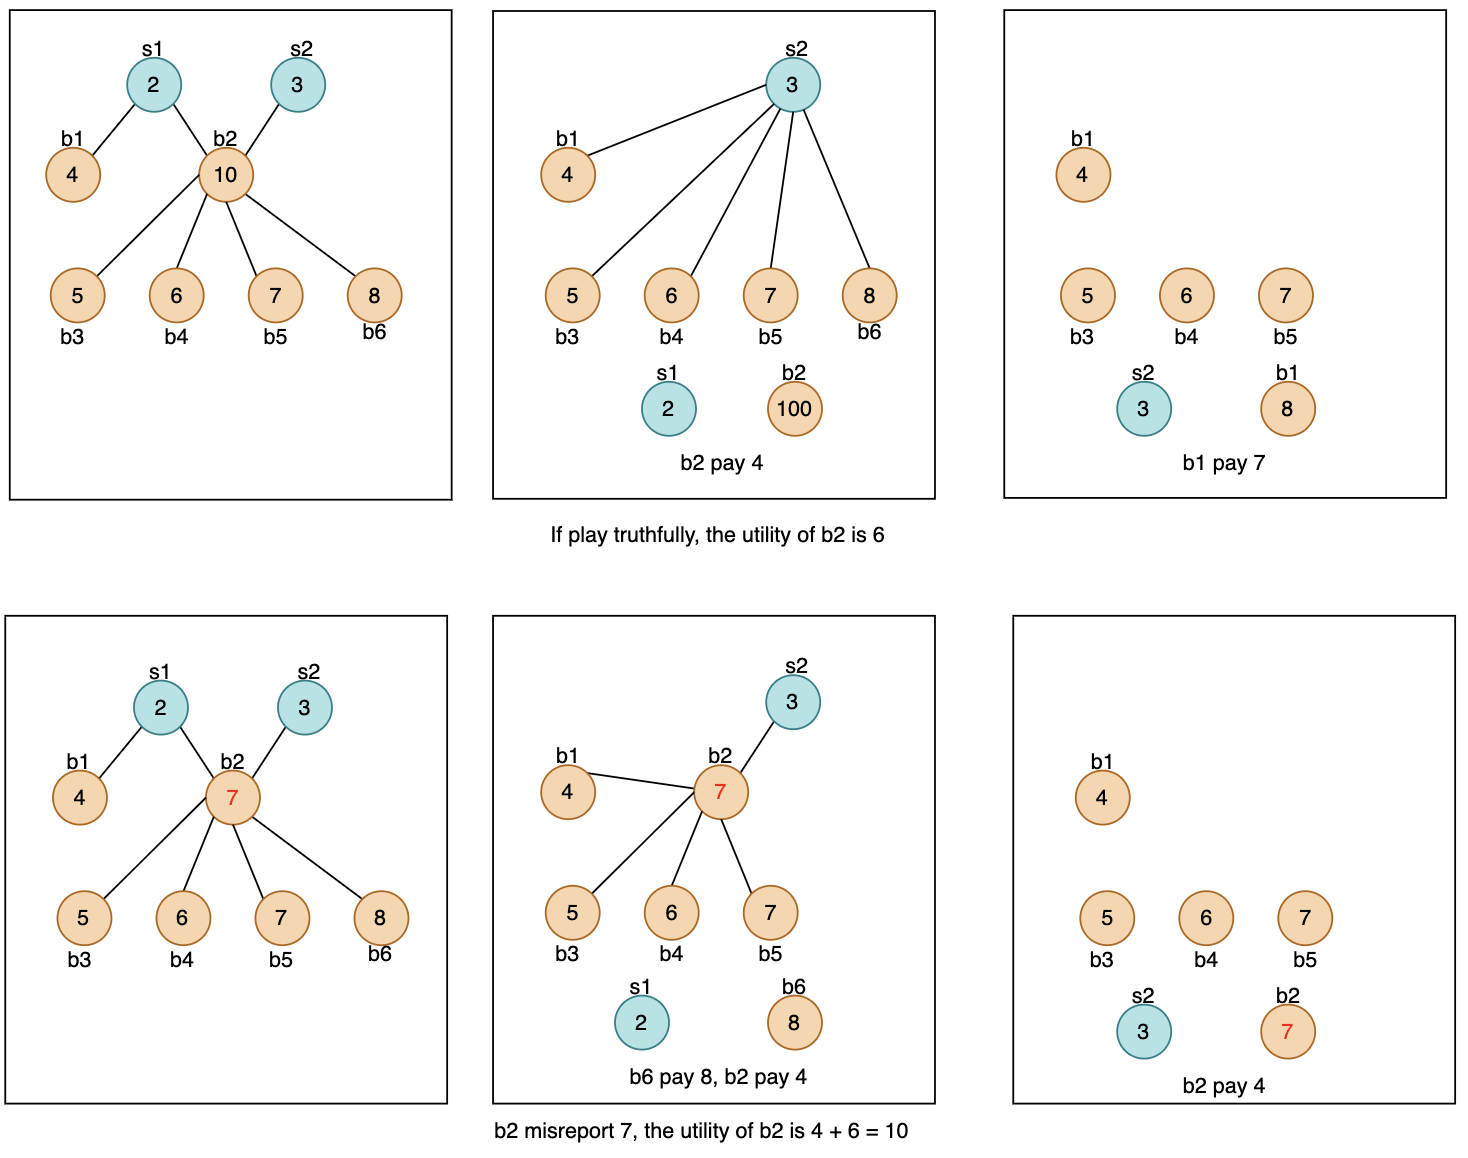
\includegraphics[width = \textwidth]{image/IDMCounter2.png}
	\caption{A run of the patched version}
	\label{fig:IDMcounter2}
\end{figure}
\subsection{DNA on Connected Network}
The only work on double auctions on social networks is Double Network Auction (DNA)\cite{DNA}. The method is an extension of McAfee's trade reduction mechanism that runs on several disjoint buyer networks. Therefore, we may reduce our model to DNA's model
by dividing the connected buyer networks into several disjoint smaller buyer networks. After that, we can use DNA to calculate the result. To achieve this, we have to make a restriction on the networks.
// TODO: restrictions
With this restriction, we can try to separate the network into different buyer groups according to the lead buyer. We proposed a potential mechanism for graph division.


\begin{tcolorbox}[title=Algorithm: Graph Division]
	\begin{enumerate}
		\item Calculate each buyer's depth by finding the minimal distance to the nearest head buyer.
		\item Remove the edge between nodes with the same level.
		\item Let each head buyer be a buyer group and keep recording each buyer group's highest valuation.
		\item Start from the deepest layer and the node with the highest valuation.
		\item Find critical paths to all the buyer groups where the node has the highest value among all the nodes on the path.
		\item Ignore the nodes have no critical path.
		\item If there's only one critical path, add all the nodes on that path to the corresponding buyer group.
		\item Otherwise, choose the path to the buyer group with the lower highest valuation.
		\item  Repeat until no new buyers can be added to a group.
		\item Randomly add the omitted buyers.
	\end{enumerate}
\end{tcolorbox}
The following is a run of the algorithm to separate a random network.
\begin{figure}
	\centering
	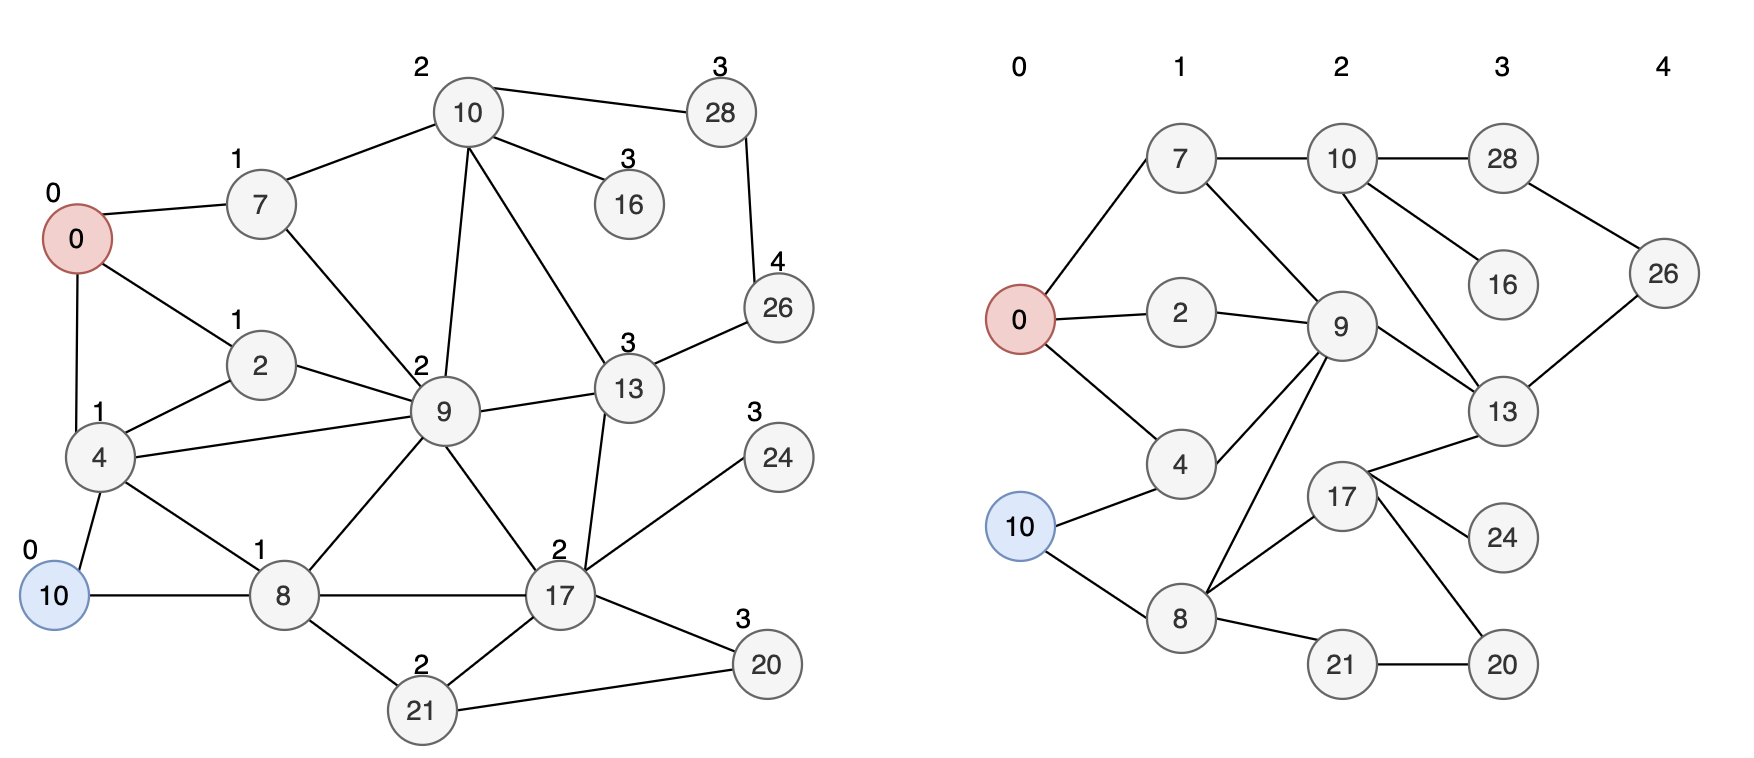
\includegraphics[width = \textwidth]{image/Graph01.png}
	\caption{First reorder the network according to the node's depth}
	\label{fig:GraphDivision1}
\end{figure}
\begin{figure}
	\centering
	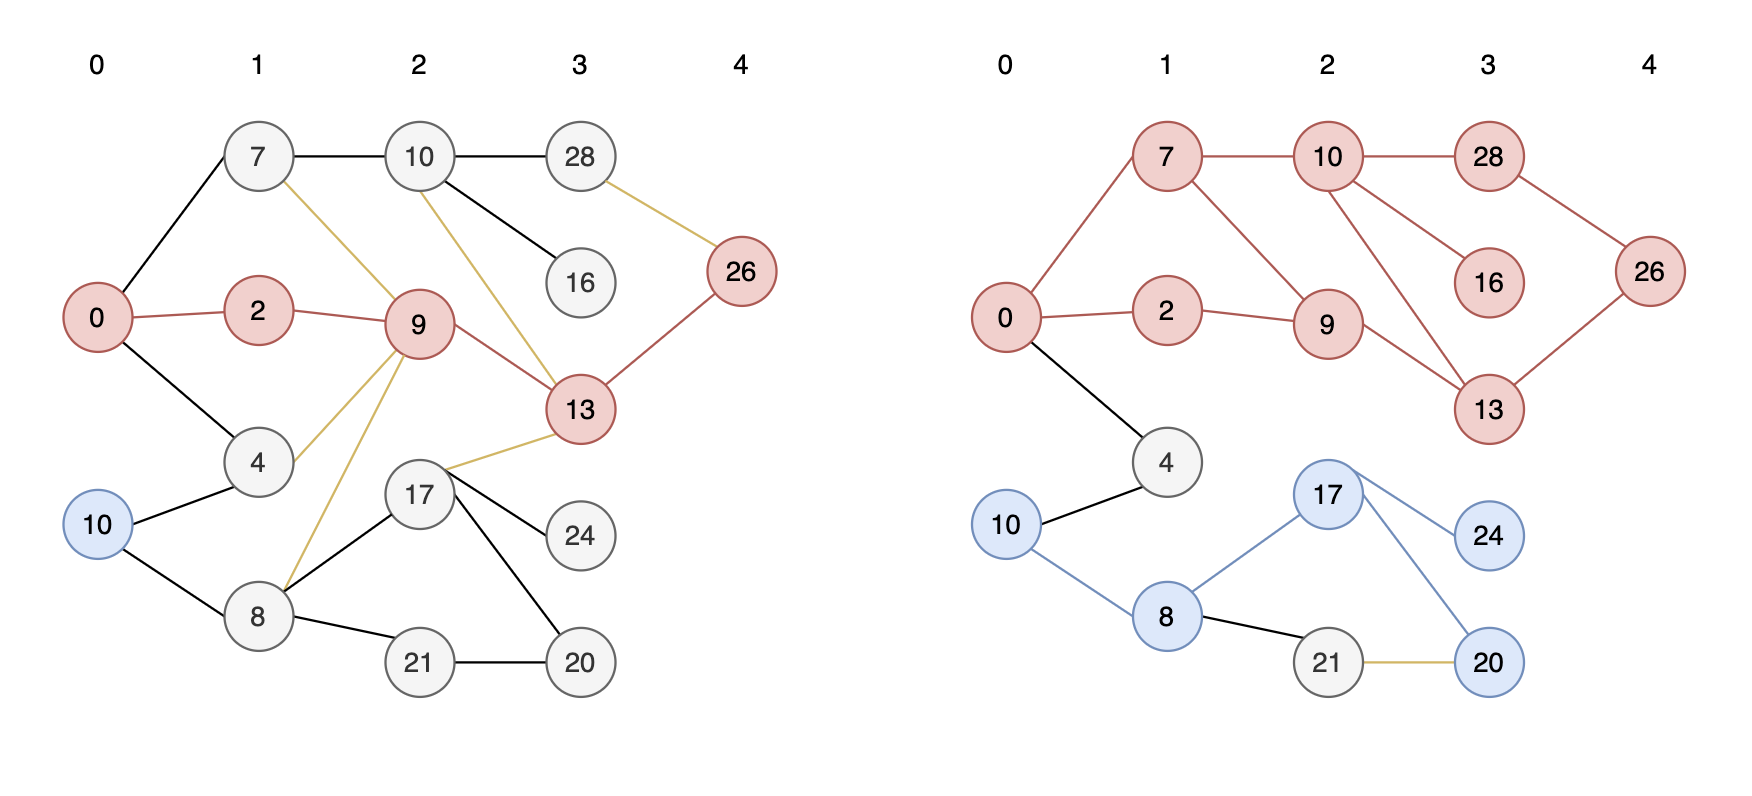
\includegraphics[width = \textwidth]{image/Graph02.png}
	\caption{Start from the deepest node and highest value, find a valid critical path and put them into the group}
	\label{fig:GraphDivision2}
\end{figure}
\begin{figure}
	\centering
	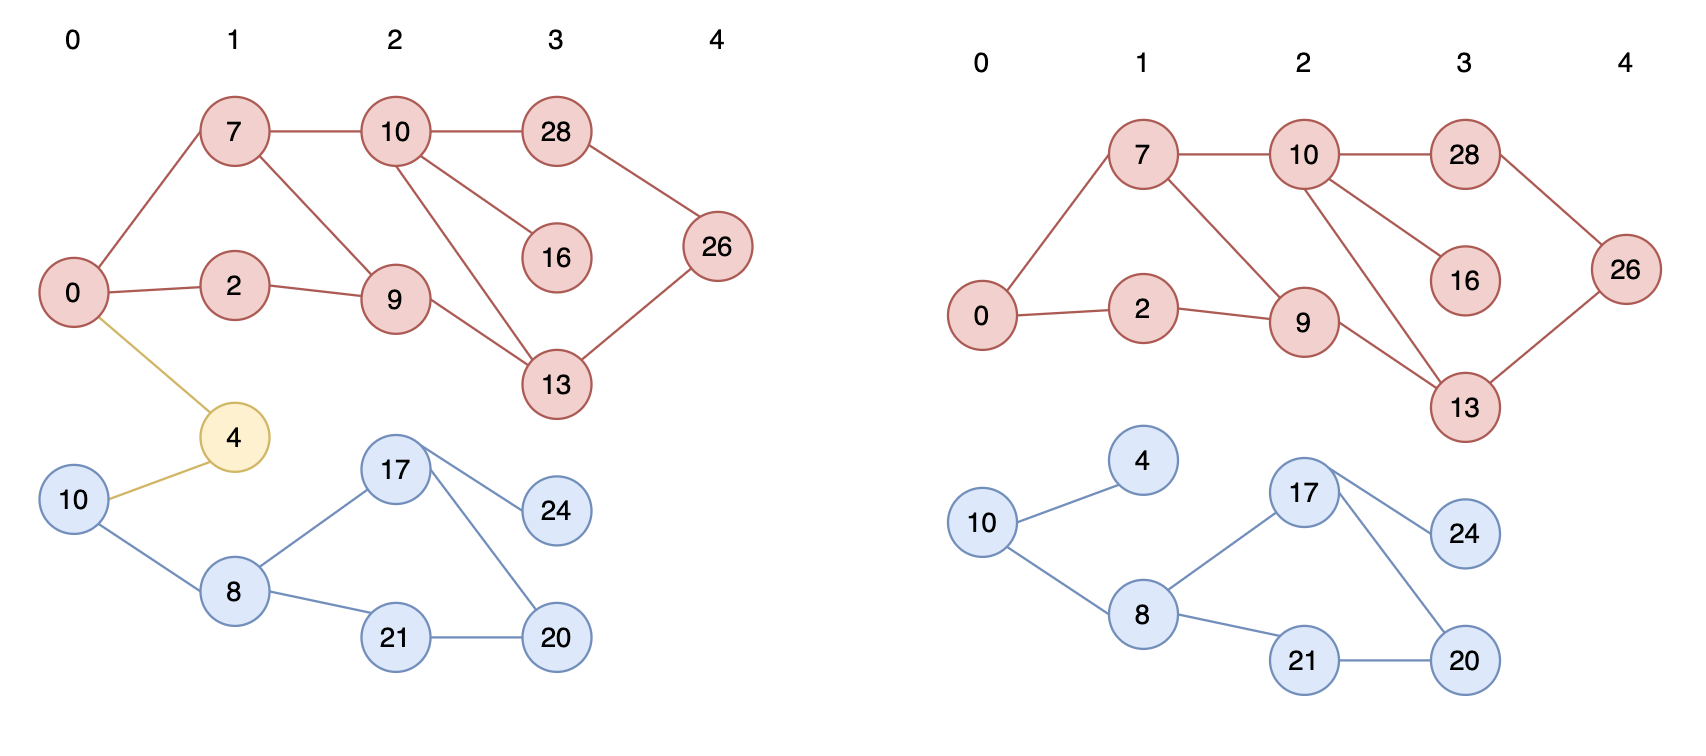
\includegraphics[width = \textwidth]{image/Graph03.png}
	\caption{When there exists multiple path, choose the group with the lower highest valuation.}
	\label{fig:GraphDivision3}
\end{figure}
However, we haven't found whether this algorithm satisfies IC.

\subsection{Club Auction}
If we add another restriction on the buyer group, there will be other appropriate mechanism. Suppose all sellers are connected to one buyer, then it can be viewed as multi-unit single auction on social network with reserved prices. We can then leverage existing IC mechanism to solve the problem. In addition, all the sellers are connected together, so the sequence of selling is not important. Therefore, we proposed Club Auction.
\begin{tcolorbox}[title=Algorithm: Club Auction]
	\begin{enumerate}
		\item Let \(\mathcal{M}\) be the multi-unit single auction mechanism that is IC.
		\item Let \(m = \) the number of sellers. For convenience, suppose that: \(|v^s_1| < |v^s_2| < \ldots < |v^s_m|\).
		\item Run \(\mathcal M\) with \(m\) items.
		\item Let \(p = \) the sum of the buyers' payments given by \(\mathcal M\).
		\item If for all \(|v^s_i| \geq \left|\frac p m\right|\), then let \(p^s = -\frac p m\) be the payment of each seller. And the allocation given by \(\mathcal M\) be the final allocation.
		\item Otherwise, let \(m = m - 1\). If \(m > 0\), go to 3.
	\end{enumerate}
\end{tcolorbox}

In figure \ref{fig:MUDAN}, it shows a run of Club Auction using MUDAN\cite{MUDAN-MUDAR} as \(\mathcal{M}\).

\begin{figure}
	\centering
	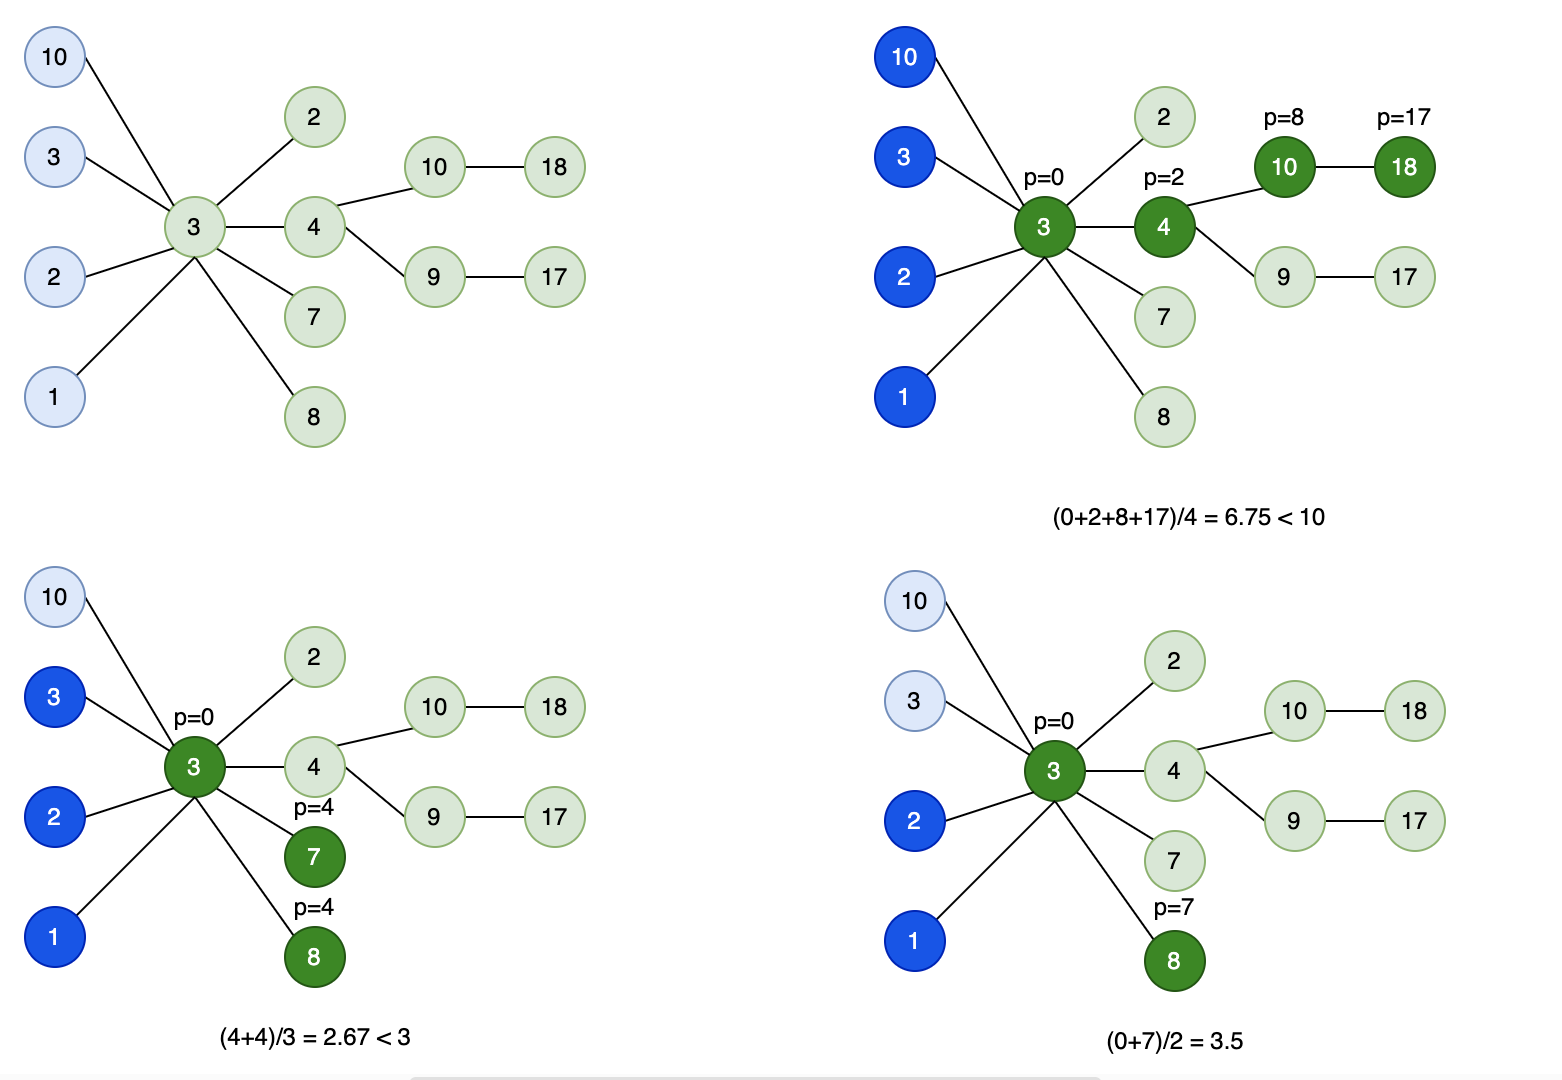
\includegraphics[width = \textwidth]{image/MUDAN.png}
	\caption{A run of Club Auction using MUDAN.}
	\label{fig:MUDAN}
\end{figure}

\begin{theorem}
	Club Auction is BB.
\end{theorem}
\begin{proof}
	Since each seller will get the average paid of all the buyers, therefore,
	\begin{align*}
		sum_{s_i \in S}P^s_i(\hat\theta, \hat\theta^s) + \sum_{b_i \in B}P_i^b(\hat\theta,\hat v^z)
		 & = m \times - \frac{p}{m} + p \\
		 & = 0
	\end{align*}
\end{proof}

\begin{theorem}
	Club Auction is IC.
\end{theorem}
\begin{proof}
	Let \(p^{b(i)}\) be the total payment given by all the buyers when there are \(i\) to be sold.
	\begin{itemize}
		\item The buyer will play truthfully since \(M\) is IC.
		\item For seller, suppose at one moment, \(i\) sellers agree on the payments and the algorithm stops.
		      \begin{itemize}
			      \item If \(|v^s_i| > \frac{p^{b(i)}}{i}\) and the seller misreports \(|v^{s*}_i| < |v^s_i| \) to get the item, then the seller's utility will be negative.
			      \item If \(|v^s_i| < \frac{p^{b(i)}}{i}\) and the seller misreports \(|v^{s*}_i| > |v^s_i| \), then the trade will failed, and the seller will not get the item. Her utility will become zero.
		      \end{itemize}
		\item Under other circumstances, the misreport will not affect the payment from the buyer. And thus, the utility for the seller will not change.
	\end{itemize}
	Therefore, the Club Auction is IC.

\end{proof}


\section{Conclusion}

In this course project, we tackled the problem of social network double auction mechanism design.
After reviewing the existing mechanism for auctions in social network, we formulated our model and set the targets.
We approached the problem in three different ways: leave and share reselling auction, club auction and DNA with graph partitions. Although our result are primitive, they provided critical insights into the problem.

\printbibliography

\end{document}
